%%%%%%%%%%%%%%%%%%%%%%%%%%%%%%%%%%%%%%%%%
% Beamer Presentation
% LaTeX Template
% Version 1.0 (10/11/12)
%
% This template has been downloaded from:
% http://www.LaTeXTemplates.com
%
% License:
% CC BY-NC-SA 3.0 (http://creativecommons.org/licenses/by-nc-sa/3.0/)
%
%%%%%%%%%%%%%%%%%%%%%%%%%%%%%%%%%%%%%%%%%

%----------------------------------------------------------------------------------------
%	PACKAGES AND THEMES
%----------------------------------------------------------------------------------------

\documentclass[c]{beamer}
%\documentclass[notes]{beamer}
\setbeamertemplate{note page}[show only notes]
\input{../OR_common.tex}
%%%%%%%%%%%%%%%%%%%%%%%%%%%%%%%%%%%%%%%%%%%%%%%%%%%%%%%%%%%%%%%%%%%%%%%%%%%%%
%%%%%%%%%%%%%%%%%%%%%%%%%%%%%%%%%%%%%%%%%%%%%%%%%%%%%%%%%%%%%%%%%%%%%%%%%%%%%
%%%%%%%%%%%%%%%%%%%%%%%%%%%%%%%%%%%%%%%%%%%%%%%%%%%%%%%%%%%%%%%%%%%%%%%%%%%%%

\title[Introduction]{Unit 2. Linear programming. The Simplex Method}

\author{Jordi Villà i Freixa}
\institute[FCTE]{
Universitat de Vic - Universitat Central de Catalunya \\
Study Abroad. Operations Research\\
\medskip
\textit{jordi.villa@uvic.cat}
}
\date{28/03-18/04, 2023}
\logo{
\includegraphics[width=.1\textwidth]{FCTE}}
\begin{document}

\begin{frame}
\titlepage
\end{frame}


\begin{frame}
    \frametitle{Preliminary}
    This course is strongly based on the monography on Operations Research by Carter, Price and Rabadi \cite{carter}, and in material obtained from different sources (quoted when needed through the slides).
\end{frame}


%%%%%%%%%%%%%%%%%%%%%%%%%%%%%%%%%%%%%%%%%%%%%%%%%%%%%%%%%%%%%%%%%%%%%%%%%%%%%
%%%%%%%%%%%%%%%%%%%%%%%%%%%%%%%%%%%%%%%%%%%%%%%%%%%%%%%%%%%%%%%%%%%%%%%%%%%%%
%%%%%%%%%%%%%%%%%%%%%%%%%%%%%%%%%%%%%%%%%%%%%%%%%%%%%%%%%%%%%%%%%%%%%%%%%%%%%

\begin{frame}
\frametitle{Learning outcomes}
\begin{itemize}
  \item Understanding the rational behind the Simplex method for LP.
  \item Understanding and practicing the algorithm in 2 variables.
  \item Recognizing the different types of results one can achieve in LP from the Simplex Method algorithm.
  \item Getting familiar with slack, surplus and artificial variables.
\end{itemize}
\end{frame}

\section{Introduction to the Simplex method for LP}

\begin{frame}
  \begin{center}
    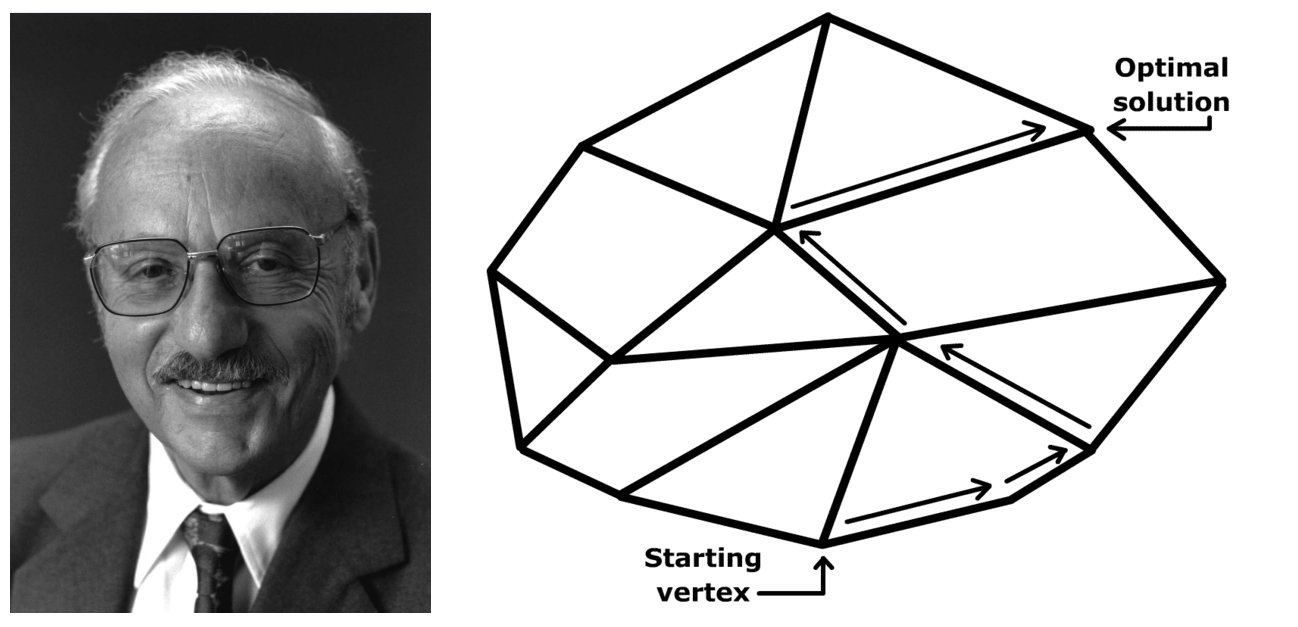
\includegraphics[width=\linewidth]{george-danzig-simplex.jpg}
  \end{center}

  Left: George Dantzig (1914-2005), the American mathematical scientist who devised linear programming and the simplex algorithm. Right: The simplex algorithm moves along the edges of the polytope until it reaches the optimum solution [Image Wikimedia Commons].
\end{frame}

\section{Preparing the LP problem for applying the Simplex method}

\begin{frame}{Classification of solutions in an LP problem}
  \begin{columns}[T]
    \begin{column}{.45\textwidth}
      \begin{center}
        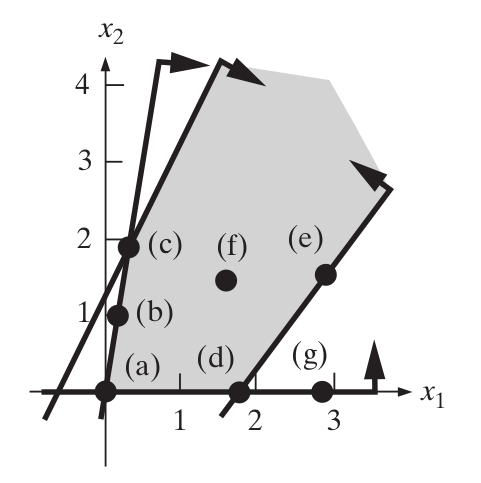
\includegraphics[width=\linewidth]{points_classification.png}
      \end{center}
    \end{column}
    \begin{column}{.45\textwidth}
      (a), (c), and (d) are both extreme points and boundary points. \\
      (b) and (e) are boundary points that are not extreme. \\
      (f) is interior because no constraint is active. \\
      (g) is neither interior nor boundary (nor extreme) because it is infeasible.\cite{rardin}
    \end{column}
  \end{columns}
\end{frame}


\begin{frame}{The standard form}

  \begin{block}{Standard form}
    For a LP with $n$ variables and $m$ constraints, the standard form is given by:
    \begin{equation*}
      \begin{aligned}
        \text{maximize } \quad & z = c_1x_1+c_2x_2 +\cdots + c_nx_n \\
        \text{subject to }\quad &
        \begin{array}{rcl}
          a_{11}x_1+a_{12}x_2+\cdots+a_{1n}x_n &= &b_1 \\
          a_{21}x_1+a_{22}x_2+\cdots+a_{2n}x_n &= &b_2 \\
          \vdots &=& \vdots\\
          a_{m1}x_1+a_{m2}x_2+\cdots+a_{mn}x_n &= &b_m \\
        \end{array}
      \end{aligned}
    \end{equation*}
    where $x_1,\ldots,x_n\geq0$ and $b_1,\ldots,b_m\geq0$
  \end{block}

Thus:
\begin{equation*}
  \begin{aligned}
    \text{maximize } \quad & z = cx \\
    \text{subject to }\quad &
    \begin{array}{c}
      Ax=b\\
      x\geq0\\
      b\geq0
    \end{array}
  \end{aligned}
\end{equation*}

\end{frame}

\begin{frame}
Of course, not always the system is proposed in this standard form, so\cite{carter}:
\begin{itemize}
  \item We need to leave a maximization problem. If the problem is to minimize the objective function, we simply multiply it by $(-1)$.
  \item In order to change inequality constraints into equality constraints we use {\it slack} variables for $\leq$ inequalities:
  \[
  3x_1+4x_2 \leq 7  \rightarrow  3x_1+4x_2+s_1 =7
  \]
  or {\it surplus} variables for $\geq$ inequalities:
  \[
  x_1+3x_2\geq 10 \rightarrow x_1+3x_2 -s_2 =10
  \]
  \item All variables should be non-negative. If some variable $x_1$ needs to be considered as unrestricted in sign, we will replace it by $x_1'-x_1''$, with $x_1',x_1''\geq 0$
\end{itemize}
\end{frame}

\section{The algebra behind the standard form}

\begin{frame}
  \begin{itemize}
 \item The system of linear equations, $Ax = b$, consists of $m$ equations and $n$
unknowns (the original decision variables plus the rest introduced to get a standard form). If the system has any solution, then $m \leq n$.
\item If $m = n$ (and if $rank (A) = m$ and $A$ is nonsingular), then 
$x = A^{-1}b$. No optimization needed!
\item If $m < n$, there are infinitely many solutions and $n -m$ degrees of freedom. 
\item A {\bf basic solution} is obtained by setting $n - m$ of the variables to zero ({\bf non-basic variables}), and solving for the remaining ({\bf basic}) $m$ variables. The number of basic solutions is $\binom{n}{n-m}=\binom{n}{m}=\frac{n!}{m!(n-m)!}$
\item Basic solutions that do not satisfy all problem constraints and non-negativity constraints are {\bf infeasible solutions}.
\item An {\bf optimal basic feasible solution} is a
basic feasible solution that optimizes the objective function. 
\end{itemize}
\end{frame}

\section{The Simplex algorithm}

\begin{frame}
 "We define
two extreme points of the feasible region (or two basic feasible solutions) as being adja-
cent if all but one of their basic variables are the same. Thus, {\em a transition from one basic
feasible solution to an adjacent basic feasible solution can be thought of as exchanging
the roles of one basic variable and one non-basic variable}. The Simplex method per-
forms a sequence of such transitions and thereby examines a succession of adjacent
extreme points. A transition to an adjacent extreme point will be made only if by doing
so the objective function is improved (or stays the same). It is a property of linear pro-
gramming problems that this type of search will lead us to the discovery of an optimal
solution (if one exists). The Simplex method is not only successful in this sense, but it
is remarkably efficient because it succeeds after examining only a fraction of the basic
feasible solutions."\cite{carter}
\end{frame}

\begin{frame}{The algorithm}
\begin{enumerate}
  \item Convert the system of inequalities to equations (using slack or surplus variables).
  \item Set the objective function to zero.
  \item Create the Simplex tableau and label active and basic variables.
  \item Select the pivot column (the one with the most negative coefficient in the zeroed objective function). This will be linked to the {\bf entering vaiable}.
  \item Select the pivot row (once divided the entry in the constant column by the ceffient in that row in the pivot column, we choose the smallest ratio). This will be linked to the {\bf leaving variable}.
  \item The pivot is the intersection between the pivot row and pivot column.
  \item Use the pivot value to make zeros in the rest of elements in the pivot column.
  \item Repeat the process from step 4, until the last row is all non-negative.
\end{enumerate}

\end{frame}

\begin{frame}{Example. Standard form}


  \begin{equation*}
    \begin{aligned}
      \text{maximize } \quad & z = 8x_1+5x_2 \\
      \text{subject to }\quad &
      \begin{array}{rcl}
        x_1 &\leq &150 \\
        x_2 &\leq &250 \\
        2x_1+x_2 &\leq &500 \\
        x_1,x_2 &\geq& 0
      \end{array}
    \end{aligned}
  \end{equation*}
We build first the standard form:
\begin{eqnarray*}
  -8x_1-5x_2+z&=&0\\
  x_1+s&=&150\\
  x_2+t&=&250\\
  2x_1+x_2+u&=&500
\end{eqnarray*}
\end{frame}

\begin{frame}{Example. The Simplex Tableau}
  We write the coefficients matrix and we identify the basic ($m=3$) and non-basic ($n-m=5-3=2$) variables:
  \begin{equation}
\begin{array}{cc}
&\\
&z \\
\rightarrow &s \\
&t \\
&u\\
\mathrm{basic}
\end{array}
%
\begin{array}{c|ccccc|c}
  z & x_1 & x_2 & s & t & u & b \\ \hline
  1 & -8 & -5 & 0 & 0 & 0 & 0 \\ \hline
  0 & 1 & 0 & 1 & 0 & 0 & 150  \\
  0 & 0 & 1 & 0 & 1 & 0 & 250 \\
  0 & 2 & 1 & 0 & 0 & 1 & 500 \\
    & \uparrow & & & & &
\end{array}
%\end{matrix}
\end{equation}
  Note that the basic variables are those for which each column is a collection of 1 and zero. We will arbitrarily assign zeros to the non-basic variables.
So a possible solution is $\boxed{P_A=(x_1=0, x_2=0)\Rightarrow z=0}$.

  The arrow marks the pivot column. We will take the pivot row by considering which is the lowest value among 150/1 and 500/2. So, the pivot row corresponds to the $s$ basic variable.
\end{frame}

% \begin{frame}{Example. Graphic solution}
%   \begin{center}
%    \includegraphics[width=0.5\linewidth]{LP7.pdf}
%   \end{center}
% \end{frame}

\begin{frame}{Example. Entering/leaving variables}

\begin{equation*}
\begin{array}{cc}
&\\
R_1+8R_2&z \\
&x_1 \\
&t \\
\rightarrow R_4-2R_2&u\\
&\mathrm{basic} \\
\end{array}
\begin{array}{c|ccccc|c}
  z & x_1 & x_2 & s & t & u & b \\ \hline
  1 & 0 & -5 & 8 & 0 & 0 & 1200 \\ \hline
  0 & 1 & 0 & 1 & 0 & 0 & 150  \\
  0 & 0 & 1 & 0 & 1 & 0 & 250 \\
  0 & 0 & 1 & -2 & 0 & 1 & 200 \\
    &  & \uparrow& & & &
\end{array}
\end{equation*}
$P_B=(150,0)$ and $z(P_B)=1200$ with $t=250$, $u=200$, $s=0$.
\end{frame}

\begin{frame}
\begin{equation*}
\begin{array}{cc}
&\\
R_1+5R_4&z \\
&x_1 \\
\rightarrow R_3-R_4&t \\
&x_2\\
&\mathrm{basic} \\
\end{array}
\begin{array}{c|ccccc|c}
  z & x_1 & x_2 & s & t & u & b \\ \hline
  1 & 0 & 0 & -2 & 0 & 5 & 2200 \\ \hline
  0 & 1 & 0 & 1 & 0 & -1 & 150  \\
  0 & 0 & 0 & 2 & 0 & 1 & 50 \\
  0 & 0 & 1 & -2 & 0 & 1 & 200 \\
    &  & & \uparrow& & &
\end{array}
\end{equation*}

\begin{equation*}
\begin{array}{cc}
&\\
R_1+5R_4&z \\
&x_1 \\
\rightarrow R_3-R_4&s \\
&x_2\\
&\mathrm{basic} \\
\end{array}
\begin{array}{c|ccccc|c}
  z & x_1 & x_2 & s & t & u & b \\ \hline
  1 & 0 & 0 & 0 & 1 & 4 & 2250 \\ \hline
  0 & 1 & 0 & 0 & -1/2 & 1/2 & 125  \\
  0 & 0 & 0 & 1 & 1/2 & -1/2 & 25 \\
  0 & 1 & 0 & 1 & 0 & 0 & 250 \\
    &  & & \uparrow& & &
\end{array}
\end{equation*}

$\boxed{P_D=(125,250)}$ and $\boxed{z(P_D)=2250}$ with $t,u=0$ (binding constraints), $s=25$ (non-binding constraint).
\end{frame}

\begin{frame}{Exercises}
  Solve, using the Simplex method, the Exercises 3 (p17) and 6 (p23) of the previous session
\end{frame}

\section{Application of SIMPLEX to non-linear problems}

\begin{frame}
  Algorithm (see example in the next page):
\begin{enumerate}
\item In $\mathbf{R}^2$, we form a triangle with vertices at $x^{[0]}$ and the two points $x^{[1]} = x^{[0]} + l_1e^{[1]}$ and  $x^{[2]} = x^{[0]} + l_2e^{[2]}$. In $\mathbf{R}^N$ the triangle becomes a simplex with $N + 1$ vertices.
\item We aim at moving ${x^{[0]}, x^{[1]}, x^{[2]},...}$ so that the triangle comes to enclose a local minimum $x_{\mathrm{min}}$ while shrinking in size.  First, the vertex of highest cost function value is moved in the direction of the {\bf triangle’s center} towards a region where we expect the cost function values to be lower. After a sequence of such moves, the triangle eventually contains in its interior a local minimum. 
\item The size of the triangle is progressively reduced until it tightly bounds the local minimum, as the vertex moves are most likely to succeed when the triangle is small enough that $F(x)$ varies linearly over the triangle region.
\end{enumerate}
\end{frame}

\begin{frame}
  \begin{center}
    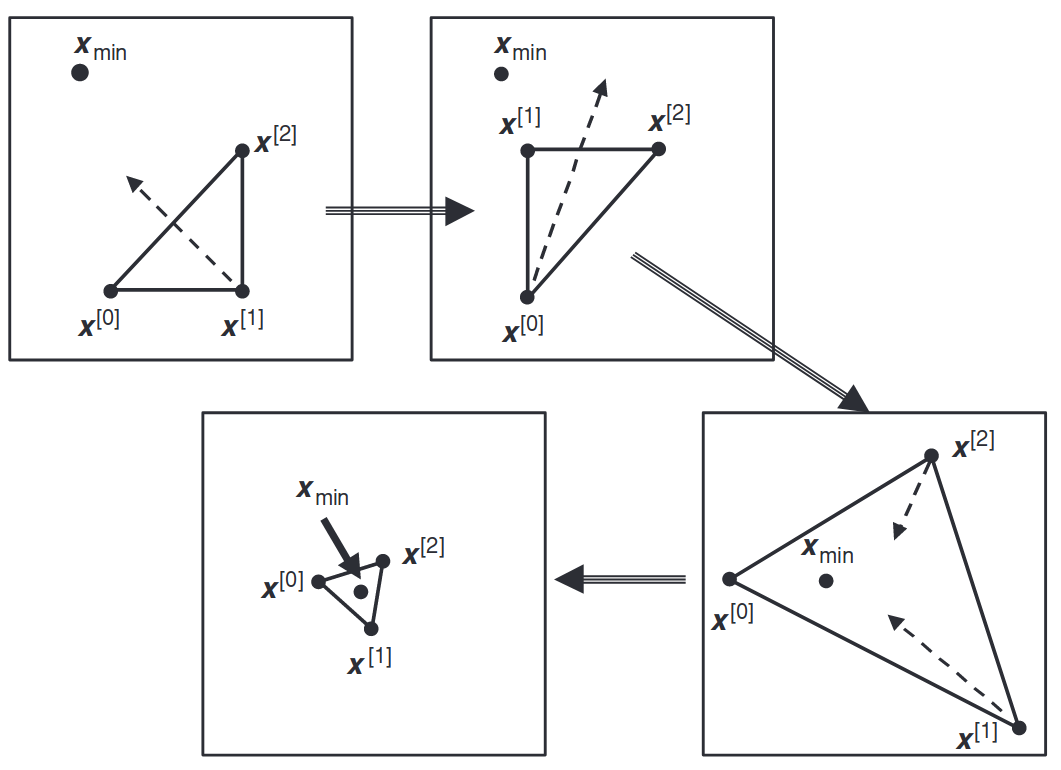
\includegraphics[width=0.7\linewidth]{simplex_nonlinear.png}
  \end{center}
  The simplex method moves the vertices of the simplex (in two dimensions, a triangle) until it contains the local minimum, and shrinks the simplex to find the local minimum (taken from \cite{beers}).
\end{frame}

\section{References}
\begin{frame}{References}
    \footnotesize
    \begin{thebibliography}{99}
    \setbeamertemplate{bibliography item}[text]
      \begin{columns}[t]
        \begin{column}{.45\textwidth}
            \bibitem{carter} Michael W. Carter, Camille C. Price, and Ghaith Rabadi. Operations Research, 2nd Edition. CRC Press.
            \bibitem{harel} David Harel, with Yishai Feldman. Algorithmics: the spirit of computing, 3rd Edition. Addison-Wesley.
            \bibitem{rardin} Ronald L. Rardin. Optimization in Operations Research, 2nd Edition. Pearson.
            \bibitem{hefferon} J. Hefferon. \href{http://joshua.smcvt.edu/linearalgebra}{Linear algebra (4th Ed)}.
        \end{column}
        \begin{column}{.45\textwidth}
            \bibitem{riley} K.F. Riley, M.P. Hobson, S.J. Bence. Mathematical Methods for Physics and Engineering (2nd Ed). McGraw Hill.
            \bibitem{nocedal} J. Nocedal, S. J. Wright. Numerical Optimization (2nd Ed). Springer.
            \bibitem{beers} Kenneth J. Beers. Numerical methods for chemical engineering: applications in Matlab. Cambridge University Press.
            \bibitem{barber} D. Barber. Bayesian reasoning and machine learning. Cambridge University Press.
        \end{column}
      \end{columns}
    \end{thebibliography}
\end{frame}
%----------------------------------------------------------------------------------------

\end{document}
